\documentclass{beamer}
\usepackage{graphicx}

% Pittsburgh is bare, but title is right justified
% Rochester is okay (just a blue background for the title)
% Singapore is good (prettier than Rochester with a very light blue)
% Boadilla is very good
% Luebeck is very good
% Warsaw is very very good
% CambridgeUS is cute
% Madrid is good
% Copenhagen is good
% Malmoe is very good

\mode<presentation>
{
  \usetheme{CambridgeUS}
}

\usepackage[english]{babel}
% or whatever

\usepackage[latin1]{inputenc}
% or whatever

\usepackage{times}
\usepackage[T1]{fontenc}
% Or whatever. Note that the encoding and the font should match. If T1
% does not look nice, try deleting the line with the fontenc.

\title{The Indian financial reforms:\\ A status report}
\author{Ajay Shah\\
http://www.mayin.org/ajayshah}

\newcommand{\fullpage}[1]{
\part{#1}
\begin{frame}
  \partpage
\end{frame}
}

\begin{document}
\begin{frame}
  \titlepage
\end{frame}

\begin{frame}
  \frametitle{Measuring outcomes}
  \begin{itemize}
  \item There are many good measures of outcomes.
  \item \textit{Example}: To measure the outcomes associated with the
    bankruptcy process, we would look at the recovery rate.
  \item \textit{Example}: To measure the outcomes associated with
    financial markets reform, we would measure various notions of
    liquidity (depth, resilience). 
  \end{itemize}
\end{frame}

\begin{frame}
  \frametitle{The outcome is not shaped by policy alone}
  \begin{itemize}
  \item In the US, securities are big, so fairly shabby financial
    markets give good liquidity.
  \item In Sri Lanka, it's very hard to make an index futures market
    liquid.
  \item Further, macroeconomic conditions matter.
  \item E.g. in a crisis, bankruptcy process would do fire sales and
    the recovery rate would go down.
  \end{itemize}

  Hence: We should measure the \textit{inputs} by policy makers. The
  outcomes do not uniquely identify the inputs.
\end{frame}

\begin{frame}
  \frametitle{What should we look for in financial reforms?}
  Three components:

  \begin{enumerate}
  \item Legal foundations
  \item Markets
  \item Financial firms
  \end{enumerate}
\end{frame}

\begin{frame}
  \frametitle{Legal foundations}
  \begin{enumerate}
  \item Governance of financial agencies
  \item Legislative, executive, judicial processes
  \item Consumer protection
  \item Micro-prudential regulation
  \item Development
  \item Capital controls
  \item Resolution 
  \item Financial redress
  \item Monetary policy
  \item Public debt management
  \item Financial regulatory agency
  \item Council of regulators for systemic risk regulation
  \item Systemic risk data centre
  \item Appellate Tribunal
  \item SOEs as ordinary companies
  \item Ministry of Finance restructuring
  \end{enumerate}
\end{frame}
\begin{frame}
  \frametitle{Markets}
  \begin{enumerate}
  \item Equities
  \item Bond-Currency-Derivatives Nexus
  \item Commodities
  \end{enumerate}
\end{frame}
\begin{frame}
  \frametitle{Financial firms}
  \begin{enumerate}
  \item Banks
  \item Payments
  \item Insurance
  \item Mutual funds
  \item Pensions.
  \end{enumerate}
\end{frame}

\begin{frame}
  \frametitle{The Indian story on legal foundations}
  \begin{itemize}
  \item Fairly shabby beginning
  \item Expert committee reports -- Percy Mistry, Raghuram Rajan,
    D. Swarup, U. K. Sinha, some others.
  \item FSLRC: Volume 1 with concepts and arguments, and version 1.0
    of Indian Financial Code
  \item Version 1.1 of Indian Financial Code: A mature model law.
  \end{itemize}
\end{frame}

\begin{frame}
  \frametitle{State of progress}
  \begin{enumerate}
  \item RBI CPI inflation targeting
  \item Monetary policy committee
  \item Financial Sector Regulatory Appointment Search Committee (FSRASC).
  \item Merged FMC into SEBI
  \item Moved capital controls regulation-making power for non-debt
    flows to MOF from RBI.
  \item Budget 2015: Setup PDMA, shift bond market from RBI to SEBI:
    Rolled back.
  \item MOF setup five `Task Forces' for setting up RC (M. Damodaran), FDMC
    (Subir Gokarn), FRA (D. Swarup), PDMA (D. Swarup), FSAT (Justice
    Sodhi).
  \item RC draft law on MOF website.
  \item Some movement on FDMC.
  \item 4 October 2016: Revival of the PDMA project.
  \end{enumerate}
\end{frame}

\begin{frame}
  \frametitle{Markets}
  \begin{description}
  \item[Equities] ~\\
    \begin{enumerate}
    \item Decent foundations; one key piece missing -- securities
      lending.
    \item Mistakes: margins, time of day, taxation of
      non-residents. 
    \item Decent liquidity
    \item Losing ground to the overseas market.
    \item Badly need better processes at SEBI and RBI.
    \end{enumerate}
  \item[Bond-Currency-Derivatives Nexus] ~\\
    \begin{enumerate}
    \item Mostly faulty.
    \item INR is a big market, that's giving liquidity.
    \item Bond market is mostly broken.
    \end{enumerate}
  \item[Commodity futures] ~\\
    \begin{enumerate}
    \item Commodity futures merged into the main financial market
      system, \textit{de jure} but not \textit{de facto}.
    \end{enumerate}
  \end{description}
\end{frame}

\begin{frame}
  \frametitle{Financial firms}
  \begin{description}
  \item[Banks] Entry barriers, inefficiencies, SOE domination. Fails
    on growth, stability, inclusion.
  \item[Payments] Captured by banks.
  \item[Insurance] Problems of consumer protection, concerns about
    soundness of LIC.
  \item[Mutual funds] Working reasonably well; need to strengthen SEBI
    processes.
  \item[Pensions] Early foundations of NPS laid, now need to see this
    through in its original vision.
  \end{description}
\end{frame}

\begin{frame}
  \frametitle{Scorecard for Legal foundations}
  \begin{center}
    {\small\begin{tabular}{lr}
      \hline
      Governance of financial agencies & 33 \\
      Legislative, executive, judicial processes & 33 \\
      Consumer protection & 33 \\
      Micro-prudential regulation & 33 \\
      Development & 33 \\
      Capital controls & 40 \\
      Resolution & 40 \\
      Financial redress & 40 \\
      Monetary policy & 55 \\
      Public debt management & 40 \\
      Financial regulatory agency & 40 \\
      Council of regulators for systemic risk regulation & 40 \\
      Systemic risk data centre & 40 \\
      Appellate Tribunal & 50 \\
      SOEs as ordinary companies & 0 \\
      Ministry of Finance restructuring & 0 \\
      \hline
      Overall &  34.3 \\
      \hline
    \end{tabular}}
  \end{center}
\end{frame}
\begin{frame}
  \frametitle{Markets}
  \begin{center}
    \begin{tabular}{lr}
      \hline
      Equities & 80 \\
      Bond-Currency-Derivatives Nexus & 20 \\
      Commodities & 40 \\
      \hline
      Overall & 48 \\
      \hline
    \end{tabular}
  \end{center}
\end{frame}
\begin{frame}
  \frametitle{Financial firms}
  \begin{center}
    \begin{tabular}{lr}
      \hline
      Banks & 30 \\
      Payments & 40 \\
      Insurance & 50 \\
      Mutual funds & 70 \\
      Pensions & 50 \\
      \hline
      Overall & 48 \\
      \hline
    \end{tabular}
  \end{center}
\end{frame}
\begin{frame}
  \frametitle{Overall}
  \begin{center}
    \begin{tabular}{lr}
      \hline
      Legal foundations & 34 \\
      Markets & 48 \\
      Financial firms & 48 \\
      \hline
      Overall & 43 \\
      \hline
    \end{tabular}
  \end{center}
\end{frame}

\fullpage{Quantification}

\begin{frame}
  \frametitle{Example: Bankruptcy reform}
  \begin{center}
    \begin{tabular}{l|p{2in}}
      \hline
      1. Get the ideas straight & BLRC v1 \\
      2. Get a good draft law & IBC dragon edition (90\%), BLRC v2 (80\%)  \\
      3. Enact a law & IBC, 2016 (70\%) \\
      4. Implement the law & We have an early stage IBBI: 10\% \\
      5. Measure outcome & Recovery rate? \\
      \hline
    \end{tabular}
  \end{center}
\end{frame}

\begin{frame}
  \frametitle{This suggests a report card}
  \begin{center}
    \begin{tabular}{lrr}
      \hline
      Component & Weight & Score \\
      \hline
      Ideas & 5 & 100 \\
      A good model law & 5 & 90 \\
      Enact the law & 10 & 70 \\
      Implement it & 10 & 10 \\
      \hline
      Overall status & 30 & \textbf{58.33} \\
    \end{tabular}
  \end{center}

  By watching the history of each component, we can make a
  \textit{time series} of an index of bankruptcy policy reform.
\end{frame}

\begin{frame}
  \frametitle{Designing a financial reforms index}
  Three components:

  \begin{enumerate}
  \item Legal foundations \\
    For all sub-components: (a) Concepts (b) Model law drafted (c) Law
    enacted (d) Law implemented.
  \item Markets \\
    For all sub-components: (a) Market infrastructure (b)
    Intermediation (c) Regulatory structure (d) Regulations (e)
    Enforcement.
  \item Financial firms. \\
    For all sub-components: (a) Licensing, entry barriers (b)
    Regulatory structure (c) Regulations (d) Enforcement.
  \end{enumerate}
\end{frame}

\fullpage{Example: Monetary policy}

\begin{frame}
  \frametitle{Monetary policy : Concepts}
  \begin{enumerate}
  \item 10/2/2007: Percy Mistry report: First proposal for inflation
    targeting. \textbf{10\%}
  \item 12/9/2008: Raghuram Rajan report: Second proposal for
    inflation targeting. \textbf{20\%}
  \item 22/3/2013: FSLRC: Full picture of inflation targeting
    RBI. \textbf{100\%}.
  \end{enumerate}
\end{frame}

\begin{frame}
  \frametitle{Monetary policy: Draft law}
  \begin{enumerate}
  \item 22/3/2013: FSLRC v1: A first complete monetary policy draft
    law. \textbf{90\%}.
  \item 23/7/2015: IFC v1.1. \textbf{100\%}.
  \end{enumerate}
\end{frame}

\begin{frame}
  \frametitle{Monetary policy: Law enacted}
  \begin{enumerate}
  \item 20/2/2015: Monetary policy framework agreement. \textbf{20\%}.
  \item 28/2/2016: RBI Act amended with IT and MPC. \textbf{100\%}.
  \end{enumerate}
\end{frame}

\begin{frame}
  \frametitle{Monetary policy: Law enforced}
  \begin{enumerate}
  \item 18/10/2016: 1st MPC meeting. \textbf{20\%}.
  \end{enumerate}
\end{frame}

\begin{frame}
  \frametitle{Index of legal foundations for monetary policy}
  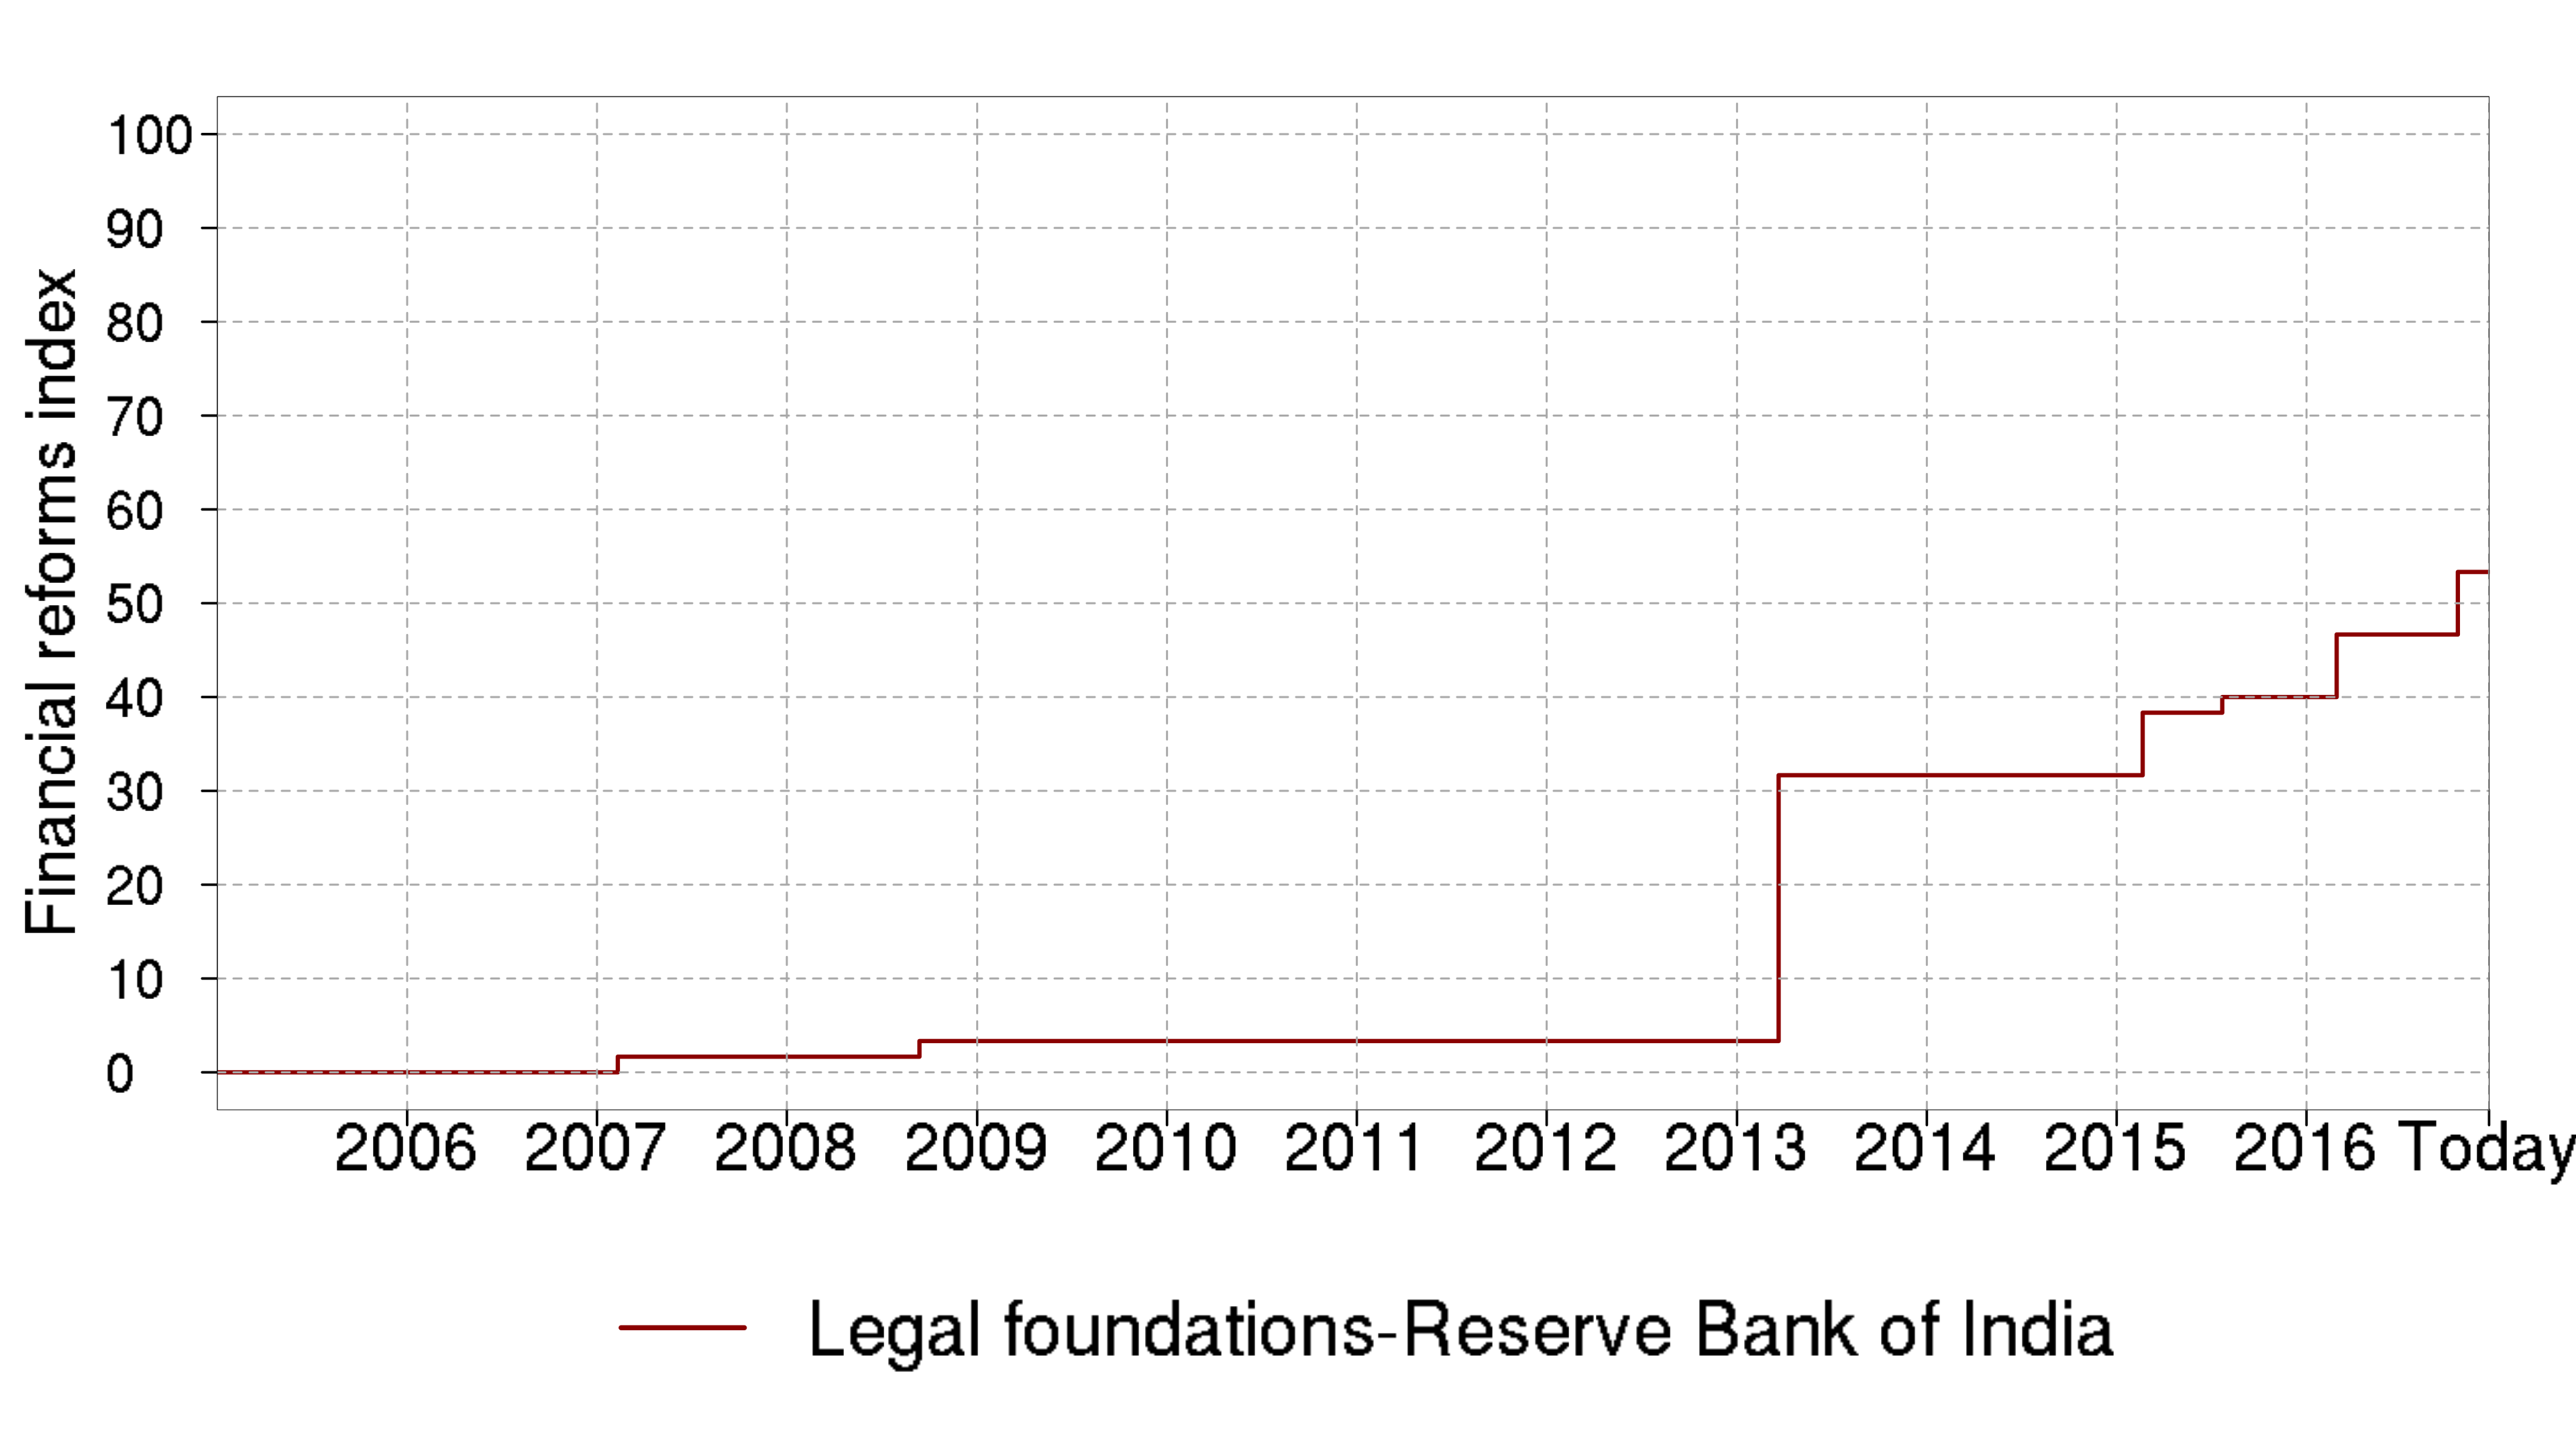
\includegraphics[width=\linewidth]{../GRAPHS/frm_index_legal_foundations_reserve_bank_of_india.png}
\end{frame}

\fullpage{Extending this to the full legal foundations}

\begin{frame}
  \frametitle{Index of legal foundations}
  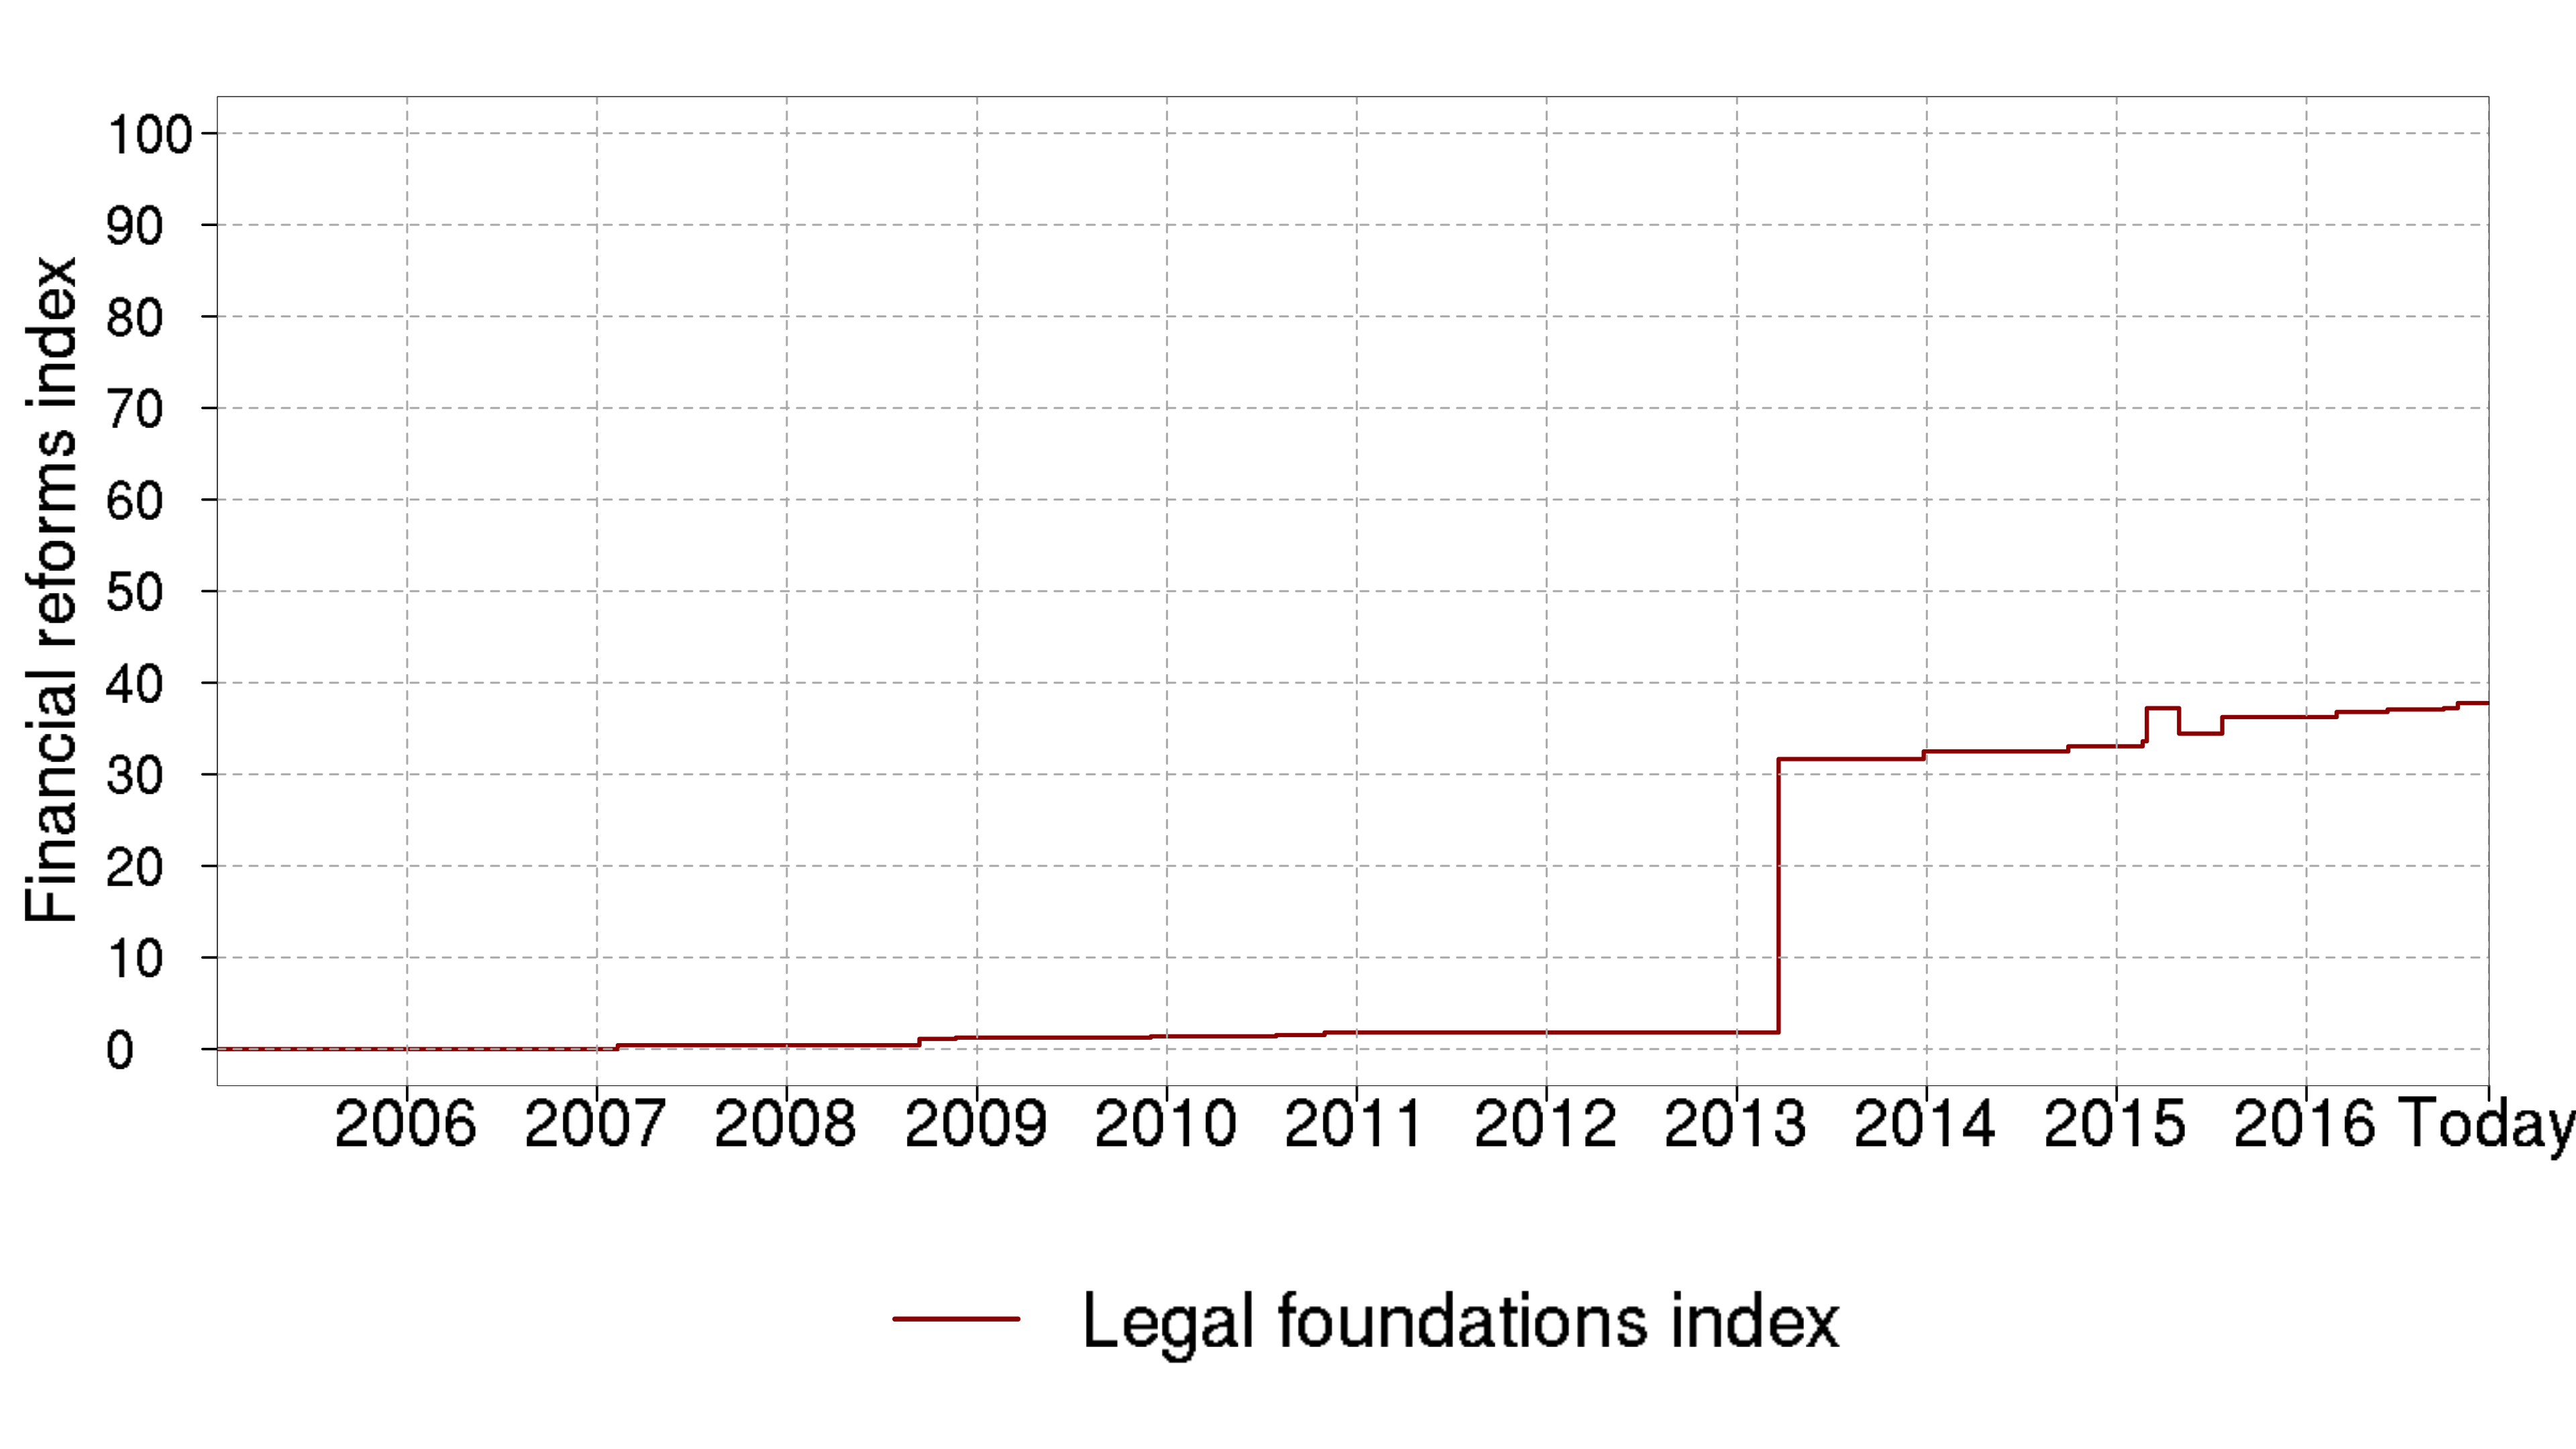
\includegraphics[width=\linewidth]{../GRAPHS/frm_index_legal_foundations.png}
\end{frame}

\begin{frame}
  \frametitle{Conclusion}
  \begin{itemize}
  \item It's useful to think systematically about the \textit{inputs},
    the financial sector reforms that will set the stage for good
    \textit{outcomes} like efficiency, inclusion, stability.
  \item In each sub-component, this requires a chronology, an economic
    history.
  \item We will soon release an R program and associated JSON file
    format through which such information systems can be created and
    manipulated.
  \end{itemize}
\end{frame}

\begin{frame}
  \hfill\mbox{\large Thank you.} 

  ~\\

  \hfill\mbox{\large http://ajayshahblog.blogspot.com}

\end{frame}

\end{document}
